\subsubsection{Simulation of the $x_{\mathrm{I}}$ and $y_{\mathrm{I}}$ Controllers}
Simulations shown in this section include the position and velocity $x_{\mathrm{I}}$ controller, as the $y_{\mathrm{I}}$ is identical. The simulations presented depict the response of the controller subjected to a step input reference signal and a corresponding simulation showing the related control action of the controller. 

In \autoref{fig:velocityControllersXY} the translational velocity controller, $\dot{x}_{\mathrm{I}}$, is subjected to a step input reference signal of \SI{1}{m s^{-1}} at time \SI{0}{s}. This yields an settling time of approximately \SI{6}{s}, when considering an error band of 5 percent. The overshoot is 15 percent. In \autoref{fig:velocityControllersXYAction} the corresponding control action is shown.

\begin{minipage}{\linewidth}
    \begin{minipage}{0.46\linewidth}
        \begin{figure}[H]
            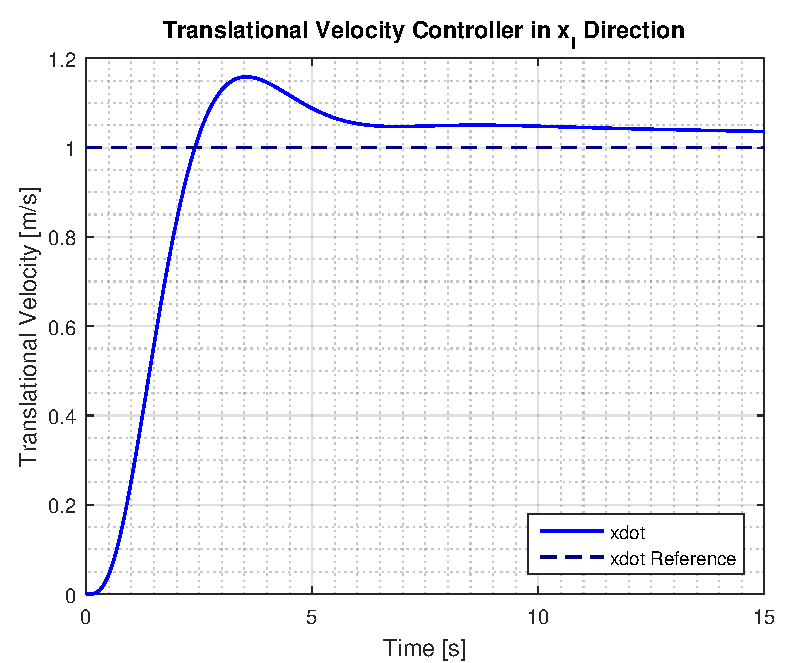
\includegraphics[scale=.5]{figures/velocityControllersXY}
            \centering			
            \captionof{figure}{Translational velocity controller step response. The control system is subjected to a step input reference signal of \SI{1}{m s^{-1}} in the $x_{\mathrm{I}}$ direction at time \SI{0}{s}.}
            \label{fig:velocityControllersXY}
        \end{figure}
    \end{minipage}
    \hspace{0.03\linewidth}
    \begin{minipage}{0.46\linewidth}
        \begin{figure}[H]
            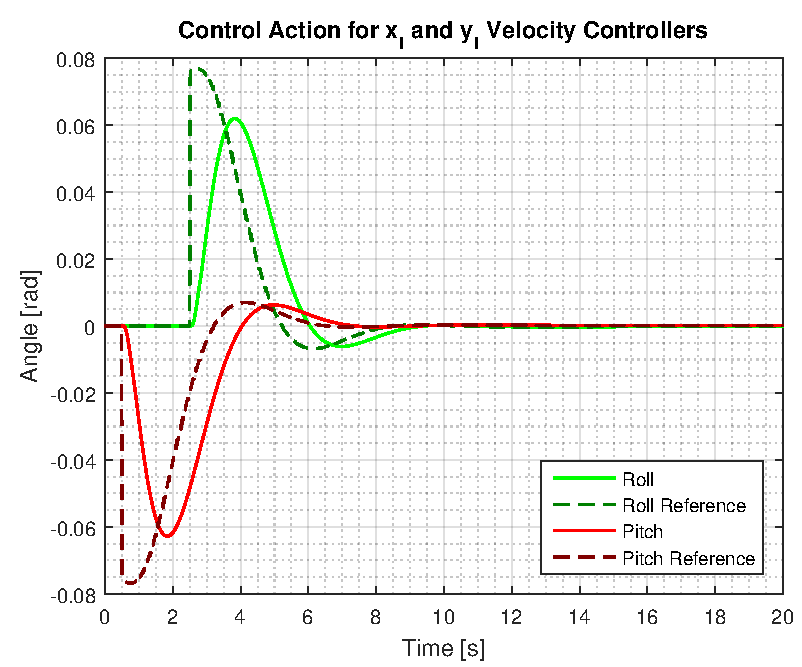
\includegraphics[scale=.5]{figures/velocityControllersXYAction}
            \centering
            \captionof{figure}{Control action required to achieve the velocity response in \autoref{fig:velocityControllersXY}, together with the the pitch response of the inner attitude controller.}
            \label{fig:velocityControllersXYAction}
        \end{figure}
    \end{minipage}
\end{minipage}

In \autoref{fig:positionControllersXY}, the translational velocity controllers, $x_{\mathrm{I}}$, is subjected to a step input reference signal of \SI{1}{m s^{-1}} at time \SI{0}{s}. It yields a settling time of approximately \SI{5}{s} and a overshoot of 2 percent. As the position controllers are designed to have a closed loop bandwidth which is three times lower than the velocity bandwidth, a larger settling time is expected. However, as the overshoot is small compared to the velocity controller, the settling time becomes lower.%and the settling time has an error band

\begin{minipage}{\linewidth}
    \begin{minipage}{0.46\linewidth}
        \begin{figure}[H]
            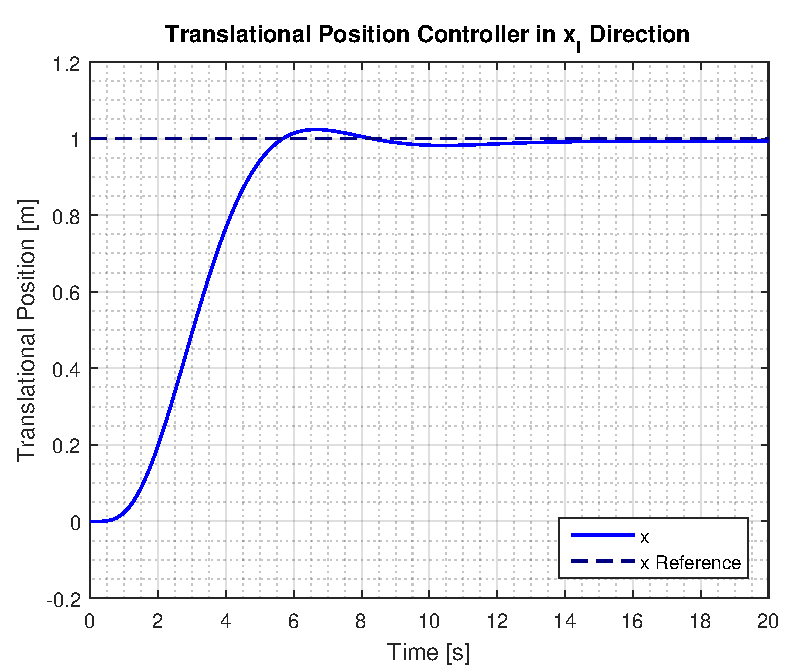
\includegraphics[scale=.5]{figures/positionControllersXY}
            \centering			
            \captionof{figure}{Step response of the position controller. The system is subjected to a step input reference signal of \SI{1}{m} in the $x_{\mathrm{I}}$ direction, at time \SI{0}{s}.}
            \label{fig:positionControllersXY}
        \end{figure}
    \end{minipage}
    \hspace{0.03\linewidth}
    \begin{minipage}{0.46\linewidth}
        \begin{figure}[H]
            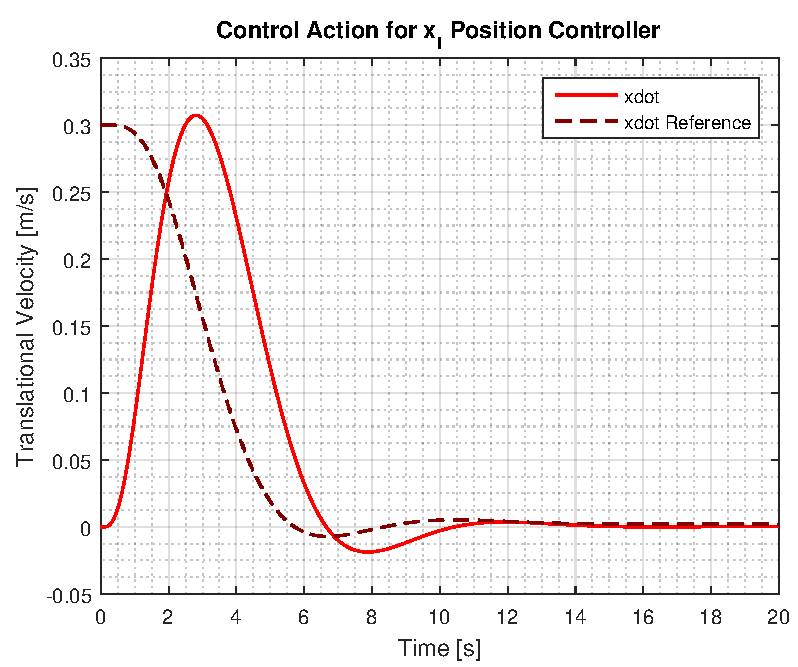
\includegraphics[scale=.5]{figures/positionControllersXYAction}
            \centering
            \captionof{figure}{Control action required to achieve the position response in \autoref{fig:positionControllersXY}, together with the response of the inner velocity controller.}
            \label{fig:positionControllersXYAction}
        \end{figure}
    \end{minipage}
\end{minipage}

The controller for the translational velocity and positioning in $x_{\mathrm{I}}$ and $y_{\mathrm{I}}$ direction have been designed and simulated. The $z_{\mathrm{I}}$ controller is to be designed in the following section.
